\SourcePage{675}{680}
\section{Double-logarithmic asymptotics of the vertex operator}

Once the corrections $\Gamma^{(1)}$ calculated in the preceding section become of order unity, evaluating the vertex operator calls for summing the entire infinite sequence of double-logarithmic terms of every order in $\alpha$. This problem can be solved because terms of this kind are produced only by diagrams of a particular type, while simple relations connect the contributions from diagrams of different orders.

\SourcePage{676}{681}
More precisely, as will be shown below, double-logarithmic terms arise from all diagrams of the form
\begin{equation}
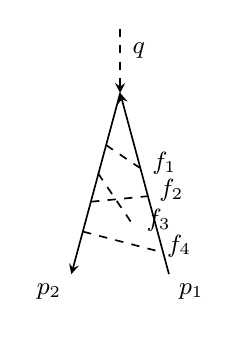
\begin{tikzpicture}[baseline=-.45ex,x=1cm,y=1cm,>=stealth,line width=.6pt,font=\small]
  \coordinate (v) at (0,1.18);
  \coordinate (l) at (-.62,-1.12);
  \coordinate (r) at (.62,-1.12);
  \draw[dashed,->] (0,2.00)--(v);
  \draw[->] (v)--(l);
  \draw[->] (r)--(v);
  \draw[dashed] (-.18,.52)--(.25,.23);
  \draw[dashed] (-.28,.16)--(.18,-.52);
  \draw[dashed] (-.37,-.20)--(.35,-.13);
  \draw[dashed] (-.47,-.58)--(.45,-.82);
  \node[right] at (.03,1.72) {$q$};
  \node[below left] at (l) {$p_2$};
  \node[below right] at (r) {$p_1$};
  \node[right] at (.28,.29) {$f_1$};
  \node[right] at (.37,-.06) {$f_2$};
  \node[right] at (.21,-.44) {$f_3$};
  \node[right] at (.47,-.76) {$f_4$};
\end{tikzpicture}
\tag{136.1}
\end{equation}
and so forth, in which every photon line joins the right-hand electron line to the left-hand one; these photon lines may cross one another in any fashion.

Number the photon momenta $f_1$, $f_2$, \ldots{} according to the order of, say, the right-hand endpoints of their lines. Different diagrams of the same order then differ by a permutation of the left-hand endpoints of the photon lines. In each Feynman integral, make approximations in the numerator and denominator analogous to those made in integral (135.5), and subsequently transform the numerator by the same procedure used in deriving (135.11). The sum of all diagrams containing $n$ photon lines, which supplies the term $\sim\alpha^n$ in $\Gamma$, consequently takes the form
\begin{equation}
\Gamma^{\mu(n)}=\gamma^\mu\left(\frac{i\alpha}{2\pi^3}t\right)^n I_n,
\tag{136.2}
\end{equation}
\begin{align}
I_n={}&\sum_{\text{perm}}
\int_{\lambda^2}d^4f_1\ldots d^4f_n\times\notag\\
&\times\frac{1}{2(p_1f_1)\cdot2(p_1f_1+p_1f_2)\ldots
2(p_1f_1+\ldots+p_1f_n)}\times\notag\\
&\times\frac{1}{2(p_2f_1)\ldots2(p_2f_1+\ldots+p_2f_n)}
\times\frac{1}{f_1^2f_2^2\ldots f_n^2},
\tag{136.3}
\end{align}
where the sum extends over every permutation of the indices on the momenta $f_k$ in the products $(p_2f_k)$; for brevity, the $i0$ and $\lambda^2$ terms in the denominators have not been displayed.

Clearly, permuting in any way the indices of the factors $f_k$ in the products $(p_1f_k)$ occurring in the sum (136.3) merely renames the momenta and therefore leaves $I_n$ unchanged. We may thus extend the summation in (136.3) to every permutation of the factors $f_k$ both in the products $(p_2f_k)$ and in $(p_1f_k)$, and then divide the result by $n!$.

\SourcePage{677}{682}
We now use the important identity
\begin{equation}
\sum_{\text{perm}}\frac{1}{a_1(a_1+a_2)\ldots(a_1+a_2+\ldots+a_n)}
=\frac{1}{a_1}\frac{1}{a_2}\ldots\frac{1}{a_n},
\tag{136.4}
\end{equation}
in which the summation is over permutations of the indices $1$, $2$, \ldots, $n$\footnote{For $n=2$ the identity is immediate, and its generalization follows readily by induction from $n$ to $n+1$.}. Applying this identity twice reduces the sum of integrals to a product of $n$ identical integrals of the form (135.19) (or (135.26)), and hence
\begin{equation}
I_n=I_1^n/n!.
\tag{136.5}
\end{equation}
Substitution into (136.2), followed by summation of $\Gamma^{(n)}$ over $n=0$, $1$, $2$, \ldots, finally gives
\begin{equation}
\Gamma^\mu(p_2,p_1;q)=\gamma^\mu\exp\left(\frac{ie^2}{2\pi^3}tI_1\right).
\tag{136.6}
\end{equation}

In particular, using $I_1$ from (135.22) yields the double-logarithmic asymptotic form of the vertex operator with virtual electron endpoints:
\begin{equation}
\Gamma^\mu(p_2,p_1;q)=\gamma^\mu\exp\left\{-\frac{\alpha}{2\pi}
\ln\frac{|q^2|}{|p_1^2|}\ln\frac{|q^2|}{|p_2^2|}\right\},
\qquad |q^2|\gg|p_1^2|,\ |p_2^2|\gg m^2
\tag{136.7}
\end{equation}
(\emph{V.~V.~Sudakov}, 1956).

Using instead $I_1$ from (135.29), we obtain the asymptotic form of the vertex operator for real electron endpoints:
\begin{equation}
\Gamma^\mu(p_2,p_1;q)=\gamma^\mu\exp\left\{-\frac{\alpha}{4\pi}
\left(\ln^2\frac{|q^2|}{m^2}+4\ln\frac{|q^2|}{m^2}\ln\frac{m}{\lambda}\right)\right\},
\qquad |q^2|\gg p_1^2=p_2^2=m^2
\tag{136.8}
\end{equation}
The factor by which $\Gamma^\mu$ differs from its unperturbed value $\gamma^\mu$ also specifies the departure of the electron-scattering amplitude in an external field from its Born value. The scattering cross section is therefore
\begin{equation}
d\sigma=d\sigma_{\text{B}}\exp\left\{-\frac{\alpha}{2\pi}
\left(\ln^2\frac{|q^2|}{m^2}+4\ln\frac{|q^2|}{m^2}\ln\frac{m}{\lambda}\right)\right\}.
\tag{136.9}
\end{equation}

Eliminating the infrared divergence, however, also requires multiplication of this expression by the sum of the probabilities for emitting different numbers of soft photons whose energies do not exceed a certain small $\omega_{\max}$; that is, it must be multiplied by (see (122.2))
\begin{equation}
1+\int_0^{\omega_{\max}}dw_\omega
+\frac{1}{2!}\int_0^{\omega_{\max}}dw_{\omega_1}
\int_0^{\omega_{\max}}dw_{\omega_2}+\ldots
=\exp\left\{\int_0^{\omega_{\max}}dw_\omega\right\}.
\tag{136.10}
\end{equation}

\SourcePage{678}{683}
For the integral in the exponent we use (120.14), specifically the expression multiplying $d\sigma_{\text{el}}$. The final result is the following asymptotic formula for scattering of an electron of energy $\varepsilon$ when the momentum transfer is large:
\begin{equation}
d\sigma=d\sigma_{\text{B}}\exp\left\{-\frac{2\alpha}{\pi}
\ln\frac{|q^2|}{m^2}\ln\frac{\varepsilon}{\omega_{\max}}\right\},
\qquad |q^2|\gg m^2,\quad
\frac{\alpha}{2\pi}\ln^2\frac{\varepsilon}{m}\sim1
\tag{136.11}
\end{equation}
(\emph{A.~A.~Abrikosov}, 1956). As expected, the first-order term in $\alpha$ in the expansion of this expression agrees with (122.12).

Notice that on taking $\omega_{\max}\sim\varepsilon$, one of the logarithms in (136.11) becomes of order unity. Thus the double-logarithmic corrections cancel when the cross section includes simultaneous emission of photons with arbitrary energies\footnote{For scattering through a finite angle, the condition stated in \S~98 for a photon to be soft requires only $\omega_{\max}\ll\varepsilon$. To logarithmic accuracy, the formulas obtained here may consequently also be used when $\omega_{\max}\sim\varepsilon$.}. In the approximation being used, the exponential factor in (136.11) then becomes unity, leaving the cross section equal to its Born value, in accordance with the general statement at the end of \S~98.
